
\hypertarget{working_databases}{}
\section{Databases}
\index{databases}

All databases uses the native XML engine provided by Borland.

\subsection{Shortcuts}
\index{databases!shortcuts}

\begin{figure}[h!]
  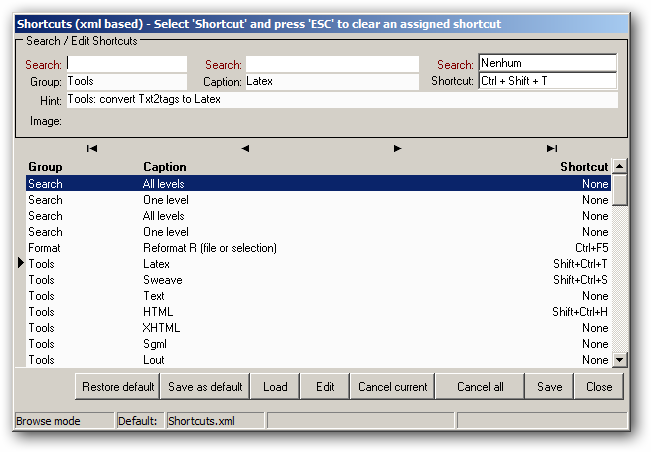
\includegraphics[scale=0.35]{./res/shortcuts_dlg.png}\\
  \caption{Shortcuts (Databases).}
  \label{fig:shortcuts_dlg_2}
\end{figure}

Read below for a brief description of available buttons (Figure \ref{fig:shortcuts_dlg_2}):

\begin{quote}
  \begin{footnotesize}
    \begin{description}
      \item[Restore default:]
        Restores the file \texttt{Shortcuts.xml} from the origin
        (InstallPath/data/data.zip). Any prior changes to the file
        \texttt{Shortcuts.xml} currently being used will be lost.
      \item[Save as default:]
        Opens the save dialog allowing you to save the file. From
        this point on, this file will be the new default shortcut.
      \item[Load:]
        Opens the open dialog allowing you to load a shortcut file.
        From this point on, this file will be the new default shortcut.
      \item[Edit:]
        Places the table in edition mode.
      \item[Cancel current:]
        Cancels any change made to the current edition.
      \item[Cancel all:]
        Cancels all changes made to the database prior to \textit{Save} or \textit{Save as default}.
      \item[Save:]
        Overwrites the text file (XML) saving all changes made to the current table.
      \item[Close:]
        Closes the dialog. All non-saved changes will be lost.
    \end{description}
  \end{footnotesize}
\end{quote}


\subsection{Completion}
\index{databases!completion}

\begin{figure}[h!]
  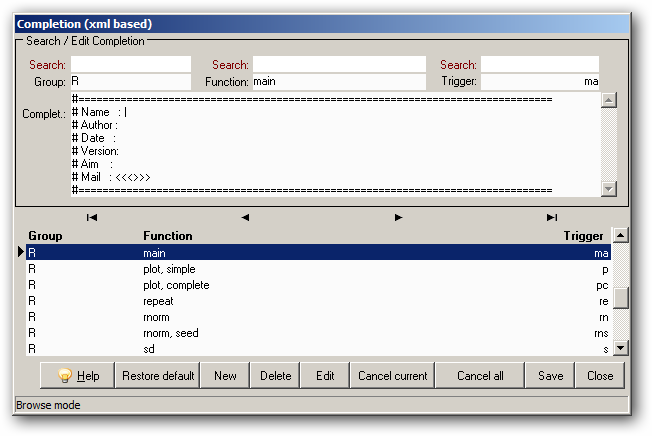
\includegraphics[scale=0.35]{./res/completion_dlg.png}\\
  \caption{Completion (Databases).}
  \label{fig:completion_dlg}
\end{figure}

This resource adds a granular level of user customization for editing
all within Tinn-R.

The completion (database based) allows the user to add functions based
on several programming languages such as \RR{}, \TeX, among others.

Read below for a brief description of available buttons (Figure \ref{fig:completion_dlg}):

\begin{quote}
  \begin{footnotesize}
    \begin{description}
      \item[Restore default:]
        Restores the file \texttt{Completion.xml} from the origin at
        (\texttt{InstallPath/data/data.zip}). Any prior change to the file
        \texttt{Completion.xml} being used will be lost.
      \item[New:]
        Places the table in insertion mode.
      \item[Delete:]
        Deletes the current registry from the table.
      \item[Edit:]
        Places the table in edition mode.
      \item[Cancel current:]
        Cancels any change made to the current edition.
      \item[Cancel all:]
        Cancels all changes made to the database prior to \textit{Save}.
      \item[Save:]
        Overwrites the text file (XML), saving all changes made to the current table.
      \item[Close:]
        Closes the dialog. All non-saved changes will be lost.
    \end{description}
  \end{footnotesize}
\end{quote}


\subsection{Comments}
\index{databases!comments}

\begin{figure}[h!]
  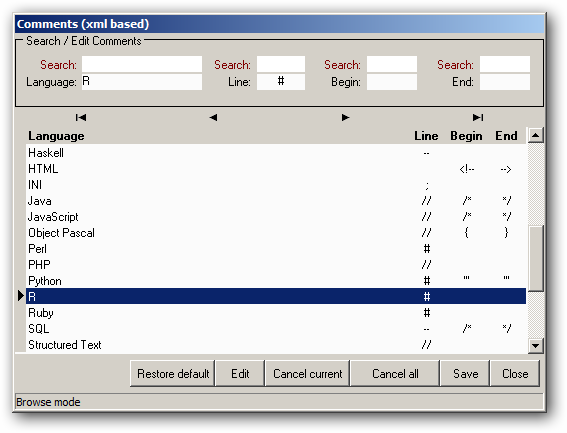
\includegraphics[scale=0.35]{./res/comments_dlg.png}\\
  \caption{Comments (Databases).}
  \label{fig:comments_dlg}
\end{figure}

The \textit{Comments} resource is very simple and allows high level
of user customization.

From version 3.0.1.0 Tinn-R automatically recognizes the
language of the file on focus. Further, inside the file
- if it is a syntax a multi-highlighter (complex syntax) - which language of
the line where the cursor (or selection) is found.

This identification is done automatically if (and only if) the option
\textit{(x) Auto detect language (recomended)} is checked. Otherwise
the user is forcing the application to use the comments of the selected language
(indicator arrow).

Selected code snippets involving more than one language will not be commented/uncommented
and a warning message is issued. That is, you must select only the snippet of a single language.

Read below a brief description of available buttons (Figure \ref{fig:comments_dlg}):

\begin{quote}
  \begin{footnotesize}
    \begin{description}
      \item[Restore default:]
        Restores the file \texttt{Comments.xml} from the origin at
        (\texttt{InstallPath/data/data.zip}). Any prior changes in the
        file \texttt{Comments.xml} currently being used will be lost.
      \item[Edit:]
        Places the table in edition mode.
      \item[Cancel current:]
        Cancels any change made to the current edition.
      \item[Cancel all:]
        Cancels all changes made to the database prior to \textit{Save}.
      \item[Save:]
        Overwrites the text file (XML) saving all changes made to the current table.
      \item[Close:]
        Closes the dialog. All non-saved changes will be lost.
    \end{description}
  \end{footnotesize}
\end{quote}


\subsection{Card (R)}
\index{R!card}
\index{databases!card (R)}

The \textit{card} was based on two \RR{} cards already published:
R/Rpad Reference Card by Tom Short and \RR{} reference card by Jonathan Baron.

\begin{figure}[h!]
  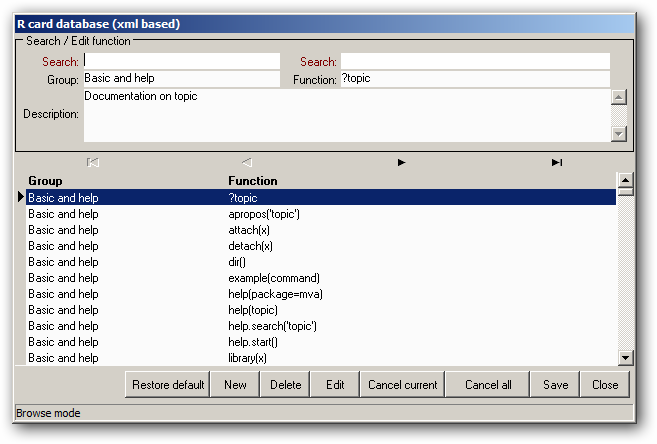
\includegraphics[scale=0.35]{./res/rcard_dlg.png}\\
  \caption{R card (Databases).}
  \label{fig:rcard_dlg}
\end{figure}

Read below a brief description of available buttons (Figure \ref{fig:rcard_dlg}):

\begin{quote}
  \begin{footnotesize}
    \begin{description}
      \item[Restore default:]
        Restores the file \texttt{Rcard.xml} from the origin at
        (\texttt{InstallPath/data/data.zip}). Any prior changes in the
        file \texttt{Rcard.xml} currently being used will be lost.
      \item[New:]
        Places the table in insertion mode.
      \item[Delete:]
        Delete the current registry from the table.
      \item[Edit:]
        Places the table in edition mode.
      \item[Cancel current:]
        Cancels any change made to the current edition.
      \item[Cancel all:]
        Cancels all changes made to the database prior to \textit{Save}.
      \item[Save:]
        Overwrites the text file (XML) saving all changes made to the current table.
      \item[Close:]
        Closes the dialog. All non-saved changes will be lost.
    \end{description}
  \end{footnotesize}
\end{quote}


\subsection{Mirrors (R)}
\index{R!mirror}
\index{databases!mirrors (R)}

The \textit{Mirrors} is an interface that allows the user to manage the repositories (or mirrors) of \RR{}.
You should always choose a repository physically closest to where you are,
so that, the Web communication tends to be faster and more efficient.

The default mirror is the University \htmladdnormallink{Wien}{http://cran.at.r-project.org/}
(Austria). Consider that this is the central mirror of CRAN.

The reasons for the Tinn-R always set a repository are two:
\begin {itemize}
   \item Prevent \RR{} keep asking which repository you want to use in each session;
   \item Workaround of intermittency (only Rterm) display the dialog for selecting the repository.
    That is, sometimes the dialog is displayed and not others. The cause of this intermittency is still unknown.
\end {itemize}

\begin{figure}[h!]
  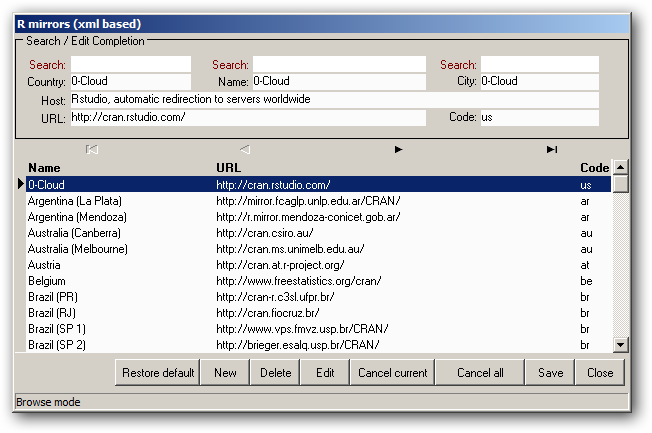
\includegraphics[scale=0.35]{./res/mirrors_dlg.png}\\
  \caption{R mirrors (Databases).}
  \label{fig:mirrors_dlg}
\end{figure}

Read below a brief description of available buttons (Figure \ref{fig:mirrors_dlg}):

\begin{quote}
  \begin{footnotesize}
    \begin{description}
      \item[Restore default:]
        Restores the file \texttt{Rmirrors.xml} from the origin at
        (\texttt{InstallPath/data/data.zip}). Any prior change to the
        file \texttt{Rmirrors.xml} while being used will be lost.
      \item[New:]
        Places the table in insertion mode.
      \item[Delete:]
        Deletes the current registry from the table.
      \item[Edit:]
        Places the table in edition mode.
      \item[Cancel current:]
        Cancels any change made during the current editing session.
      \item[Cancel all:]
        Cancels all changes made to the database prior to \textit{Save}.
      \item[Save:]
        Overwrites the text file (XML) while saving all changes made to the current table.
      \item[Close:]
        Closes the dialog. All changes not previously saved will be lost.
    \end{description}
  \end{footnotesize}
\end{quote}
